\newprob{1715431736}
{
    % active phys p282 1
    某物體受一道力作用。該力如圖示般隨時間改 變。計算該力對物體所造成的動量變化。
    \par{\par\centering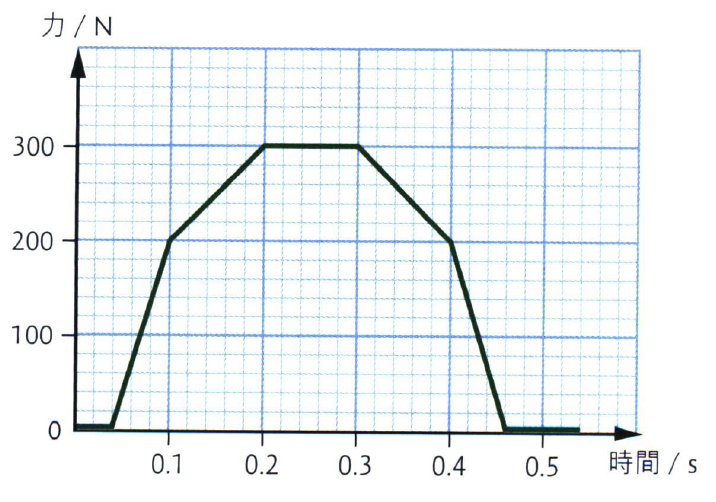
\includegraphics[width=.4\textwidth]{./img/ch5_momentum_mc_2024-05-11-21-12-39.png}\par}
    \begin{tasks}
        \task \qty{61}{kg.m.s^{-1}}
        \task \qty{80}{kg.m.s^{-1}}
        \task \qty{92}{kg.m.s^{-1}}
        \task 物體的質量不明,故未能判斷
    \end{tasks}

}{\mckey{C}
    \par{\par\centering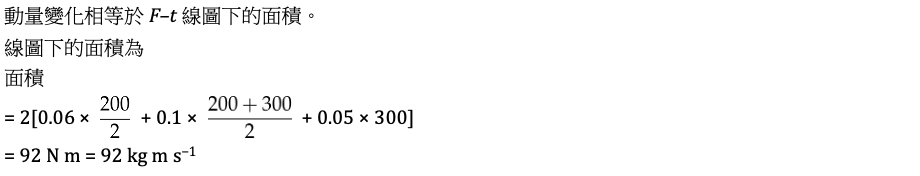
\includegraphics[width=\textwidth]{./img/ch5_momentum_mc_2024-05-11-22-59-34.png}\par}
}


\newprob{1715433281}
{
    % active phys p282 3
    有質量相同的小球A、B 兩個,小球發生對正碰 撞。碰撞前,小球 A 以速率u 移動,小球B則靜 止不動。假設碰撞為彈性碰撞,求兩球的速率。
    \begin{tasks}
        \task [] \textbf{小球}$\mathbf{A}$\tab\tab \textbf{小球} $\mathbf{B}$\vspace{1em}
        \task $u/2$ \tab\tab $u/2$
        \task $u/4$ \tab\tab $3u/4$
        \task $u/6$ \tab\tab $5u/6$
        \task 0\tab\tab $u$
    \end{tasks}

}{\mckey{D}}

\newprob{1715433459}
{
    %q6
    某物體爆炸後分裂為碎片 $X$ 和 $Y$ 。假設 $X$ 的質量 為 $Y$ 的兩倍。下列哪些敘述正確?
    \begin{statements}
        \task $X$、$Y$的速率比為$1:2$。
        \task $X$、$Y$的動量量值比為$1:2$。
        \task $X$、$Y$的動能比為$1:2$。
    \end{statements}
    \begin{tasks}
        \task 只有(1)
        \task 只有(2)
        \task 只有(1)和(3)
        \task 只有(2)和(3)
    \end{tasks}
}{\mckey{C}
    \par{\par\centering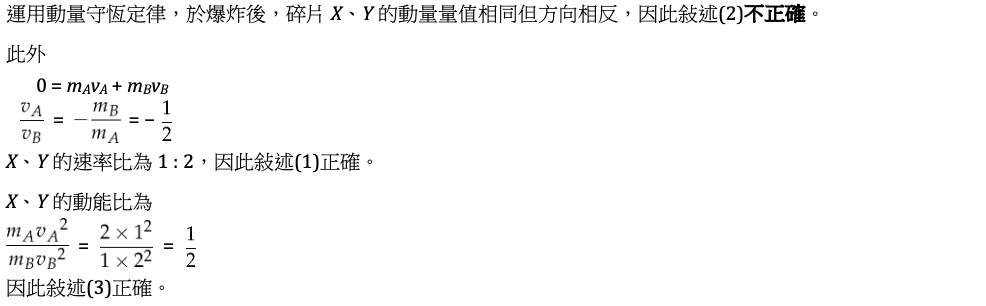
\includegraphics[width=\textwidth]{./img/ch5_momentum_mc_2024-05-11-22-50-45.png}\par}
}

\newprob{1715433583}
{
    % q7
    如圖所示,子彈射中方塊,使方塊向上升起。透 過量度方塊的最高和最低兩點之間的垂直距離, 便可計算子彈的初速度。
    \par{\par\centering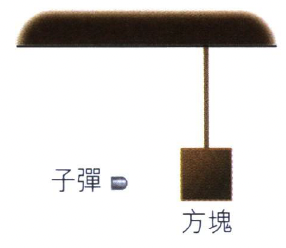
\includegraphics[width=.25\textwidth]{./img/ch5_momentum_mc_2024-05-11-21-19-51.png}\par}
    下列哪項是要得到準確結果的必要條件?
    \begin{statements}
        \task 連接方塊的繩子不可延伸。
        \task 子彈完全嵌入方塊中。
        \task 方塊的升温幅度小得可略去不計。
    \end{statements}
    \begin{tasks}
        \task 只有(1)和(2)
        \task 只有(1)和(3)
        \task 只有(2)和(3)
        \task (1), (2) 和 (3)
    \end{tasks}
}{\mckey{D}
    \par{\par\centering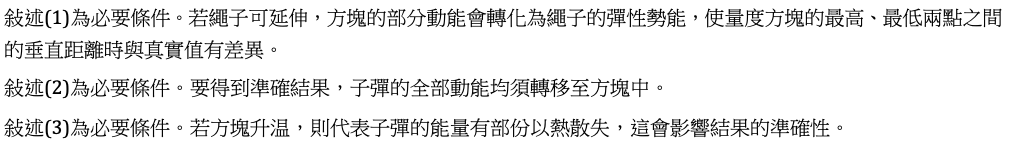
\includegraphics[width=\textwidth]{./img/ch5_momentum_mc_2024-05-11-22-50-30.png}\par}
}

\newprob{1715433680}
{
    % q8
    在光滑水平面上,兩個相同的小球P和Q起初以 相同速率移動。其後,兩球分別與小球X和Y發 生彈性碰撞。
    \par{\par\centering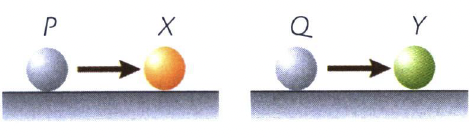
\includegraphics[width=.45\textwidth]{./img/ch5_momentum_mc_2024-05-11-21-21-41.png}\par}
    碰撞後,P變為靜止,Q則逆轉其移動方向。X、 Y 兩球中,哪一個球獲得較大動量?哪一個球獲 得較大動能?
    \begin{tasks}
        \task [] \textbf{較大動量}\tab\tab \textbf{較大動能}
        \task $X$\tab\tab$X$
        \task $X$\tab\tab$Y$
        \task $Y$\tab\tab$X$
        \task $Y$\tab\tab$Y$

    \end{tasks}

}{\mckey{C}
    \par{\par\centering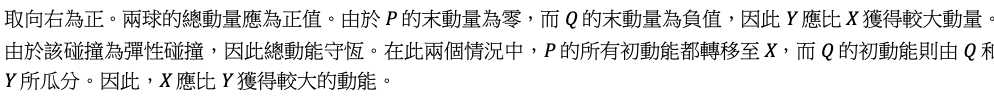
\includegraphics[width=\textwidth]{./img/ch5_momentum_mc_2024-05-11-22-50-19.png}\par}
}

\newprob{1715433863}
{
    % q9
    質量為0.7 kg的小球,從離地3 m 高處從靜止下 墜。小球着地後回彈至原來高度。假設小球與地 面的撞擊時間為0.02 s,求作用在小球上的撞擊 力。
    \begin{tasks}
        \task \qty{267}{N}
        \task \qty{384}{N}
        \task \qty{537}{N}
        \task \qty{767}{N}
    \end{tasks}

}{\mckey{C}
    \par{\par\centering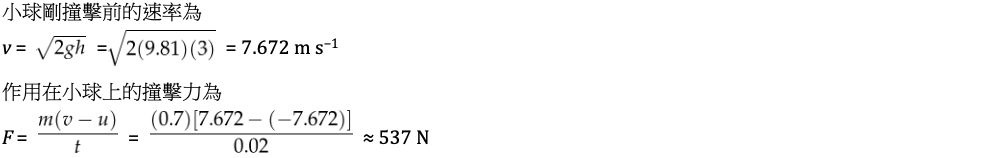
\includegraphics[width=\textwidth]{./img/ch5_momentum_mc_2024-05-11-22-50-08.png}\par}
}

\newprob{1715435297}
{
    % q10
    小球以輕繩懸掛在天花板上。偉時把小球提起高 度$h$後放手。小球抵達最低點時撞上另一個小 球,兩球黏在一起後升起。
    \par{\par\centering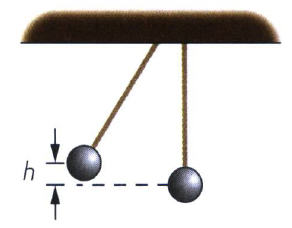
\includegraphics[width=.25\textwidth]{./img/ch5_momentum_mc_2024-05-11-21-48-45.png}\par}
    假設兩球的質量相同。求兩球升至最高點時,與 最低點的垂直距離。
    \begin{tasks}
        \task $h/4$
        \task $h/2$
        \task $h/\sqrt{2}$
        \task $h$
    \end{tasks}

}{\mckey{A}
    \par{\par\centering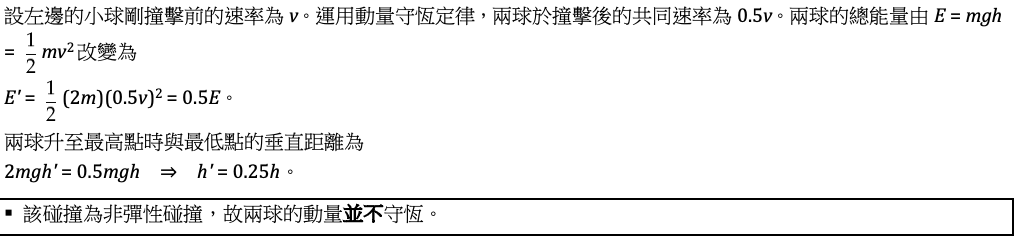
\includegraphics[width=\textwidth]{./img/ch5_momentum_mc_2024-05-11-22-49-54.png}\par}
}

\newprob{1715435392}
{
    % active phys p288 *1
    今有兩個相同的小球,在時間$t=0$的一刻,從$A$ 點沿同一水平圓形軌道以相反方向移動。兩者的 初速率分別為$2v$和3v。已知兩者曾在$t=5s$的 一刻發生彈性碰撞,兩球會於哪一刻再次於$A$點 重遇?忽略球的大小。
    \par{\par\centering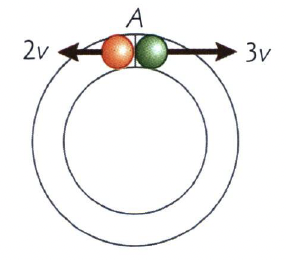
\includegraphics[width=.25\textwidth]{./img/ch5_momentum_mc_2024-05-11-21-51-19.png}\par}
    \begin{tasks}
        \task 15 s
        \task 25 s
        \task 35 s
        \task 45 s
    \end{tasks}

}{\mckey{B}
    \par{\par\centering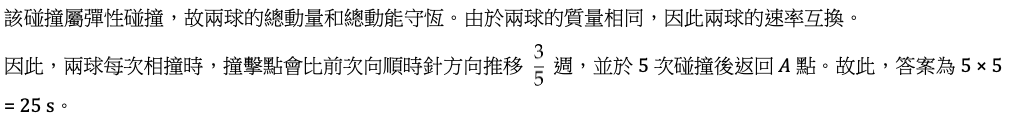
\includegraphics[width=\textwidth]{./img/ch5_momentum_mc_2024-05-11-22-49-35.png}\par}
}

\newprob{1715435432}
{
    % q2
    $A$、$B$ 兩個相同的球以互相垂直的方向移向對方, 如圖。兩球發生彈性碰撞。碰撞前,$A$的速率為 \vel{3},$B$ 的速率則為 \vel{4}。
    \par{\par\centering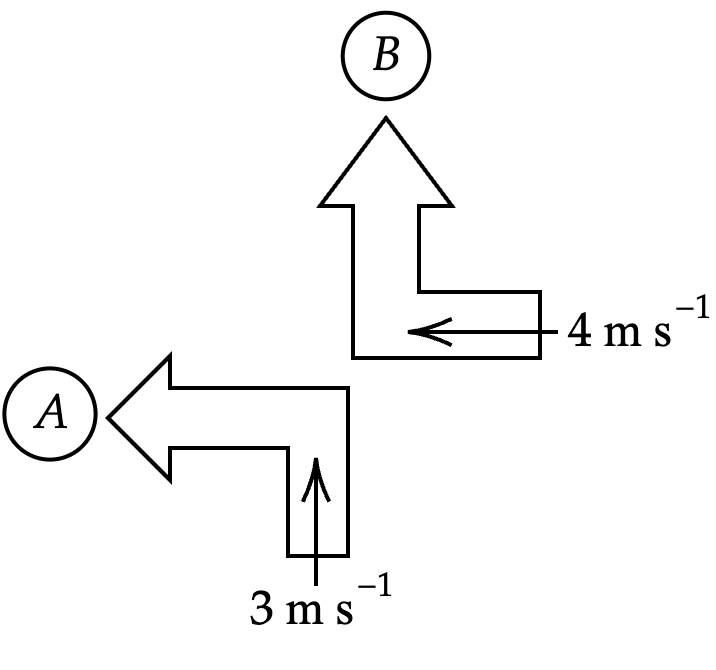
\includegraphics[width=.3\textwidth]{./img/ch5_momentum_mc_2024-05-11-21-56-50.png}\par}
    碰撞後,兩球的速率為何?
    \begin{tasks}
        \task [] \textbf{小球}$\mathbf{A}$ \tab\tab \textbf{小球}$\mathbf{B}$ \vspace{1em}
        \task \vel{1} \tab\tab \vel{1}
        \task \vel{3} \tab\tab \vel{4}
        \task \vel{4} \tab\tab \vel{3}
        \task \vel{5} \tab\tab \vel{5}
    \end{tasks}

}{\mckey{C}
    \par{\par\centering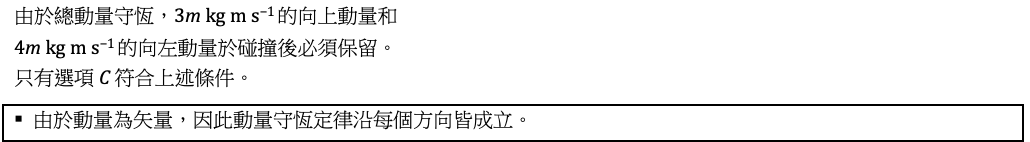
\includegraphics[width=\textwidth]{./img/ch5_momentum_mc_2024-05-11-22-49-21.png}\par}
}

\newprob{1715436077}
{
    % q3
    一個氣墊$A$與另一個起初靜止的氣墊$B$ 發生斜向 碰撞。下圖顯示兩氣墊的初速度和末速度。\bigskip
    \par{\par\centering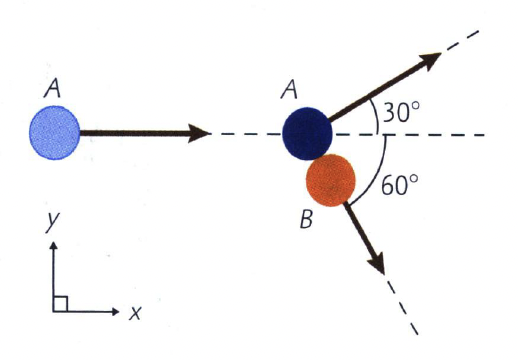
\includegraphics[width=.35\textwidth]{./img/ch5_momentum_mc_2024-05-11-22-01-38.png}\par}\bigskip
    從所得的數據中,下列哪些推斷是正確的?
    \begin{statements}
        \task 氣墊的質量相同。
        \task 氣墊的總動能守恆。
        \task 氣墊沿$x$及$y$ 方向的總動量守恆。
    \end{statements}
    \begin{tasks}
        \task 只有(1)和(2)
        \task 只有(1)和(3)
        \task 只有(2)和(3)
        \task (1), (2) 和 (3)
    \end{tasks}

}{\mckey{D}
    \par{\par\centering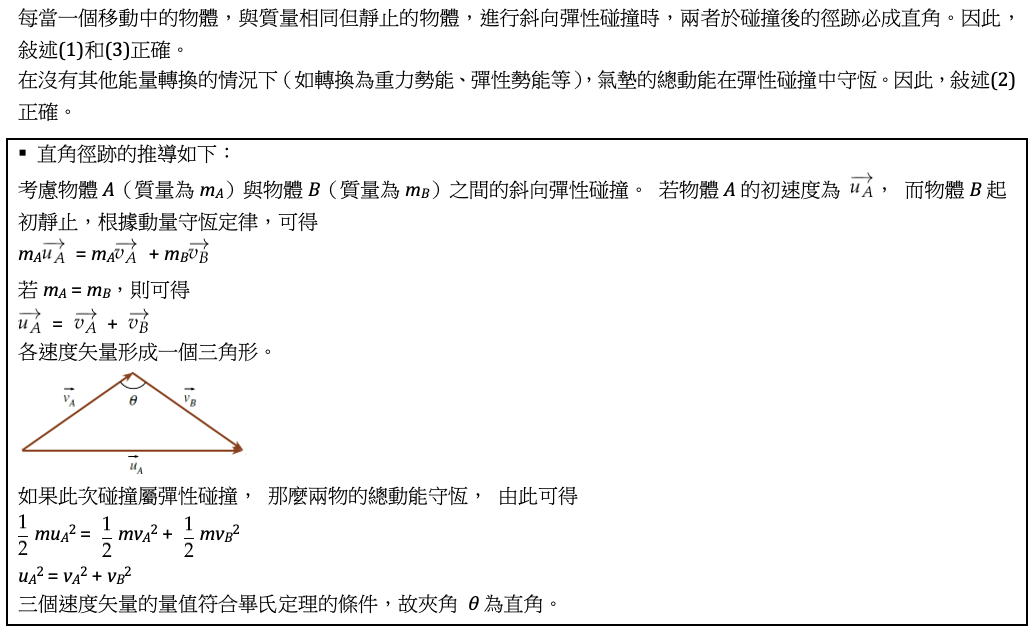
\includegraphics[width=\textwidth]{./img/ch5_momentum_mc_2024-05-11-22-49-02.png}\par}
}

